

\lettrine{H}{having discussed theories} about how our variables are connected, I here construct a research design for testing the implications of my theory. It should be remembered that we are trying to answer if a country's linkages to China affects the level of freedom of expression the population enjoys. To achieve this, it is necessary to have access to good quality data and a credible research strategy.

The first part of the chapter features a discussion of the conceptualisation and operationalisation of our two main variables: \textit{linkages} and \textit{freedom of expression}. I implicitly build this discussion on \citet{adcock_measurement_2001, gerring_what_1999}, who advocates a clear and transparent definition of the variables. Both my main variables are hard to define in a universally accepted manner, which necessitates a thorough explanation of my choices. After discussing the data, the middle part of the chapter will be concerned with the research methodology, specifically how I build the statistical models. This leaves only the end of the chapter; concerning various control-variables which must be incorporated into the model to isolate the actual effect of the linkages from other spurious causes. 

\section{The Dependent Variable: \textit{Freedom of Expression}}
I start by conceptualising and operationalising the dependent variable. There are some challenges to doing this, but the two most important points to take from this section is that: one, my definition of freedom of expression is a nuanced one; and two, that this requires me to use a subjective measure of the variable. The operationalisation will be achieved by using the Varieties of Democracy Institute's (V-Dem) Freedom of Expression and Alternative Sources of Information index \citep{coppedge_v-dem_2025}. 

\subsection{Conceptualising freedom of expression}
Freedom of expression is not at all an easy concept to define in clear terms. Everyone has a basic understanding of the intention: that every person has the right to express their opinion without any obstacles. This is not a wrong, but it quickly gets more opaque when looking at the real world.

Two of the best known definitions are the United Nation's article 19 of the \textit{Universal Declaration of Human Rights} \citeyearpar{un_general_assembly_universal_1948} and the European Union's article 11 of the \textit{Charter of Fundamental Rights of the European Union} \citeyearpar{european_parliament_charter_2012}. The first states that:
\begin{displayquote}
`Everyone has the right to freedom of opinion and expression; this right includes freedom to hold opinions without interference and to seek, receive and impart information and ideas through any media and regardless of frontiers.' \citep{un_general_assembly_universal_1948}
\end{displayquote}
The latter states that:
\begin{displayquote}
`1. Everyone has the right to freedom of expression. This right shall include freedom to hold opinions and to receive and impart information and ideas without interference by public authority and regardless of frontiers.
2. The freedom and pluralism of the media shall be respected.' \citep{european_parliament_charter_2012}
\end{displayquote}
These two are very similar in content, and we can thus read that any definition of freedom of expression should include the possibility of gathering information and imparting information without interference. They also emphasise that access to a pluralistic media environment is important. Affirming that being able to disseminate information to a wide audience factor into our basic understanding of what freedom of expression should be. This is a good start, but we need to be a bit clearer about what type of expressions we are concerned about and what restrictions are and are not proper when defining freedom of expression. 

I include four important limitations to my conceptualisation of freedom of expression. The first limitation I give freedom of expression is that it must be a political expression. Thus, we are not moving into the realm of laws against certain types of pornography \citep[pp. 6-7]{bonotti_freedom_2021} or obscene utterances. Many countries have restrictions on certain types of expressions, which they might have a good reason for having. Of course, if restrictions on non-political expression is used as a tool to silence political expression, they would still qualify as restrictions to political expression.

The second limitation is that the restrictions on freedom of expression must be \textit{de facto} rather than \textit{de jure}. If there are no formal restrictions, but the restrictions of expression still take place, it should count as a restriction of the freedom of expression. On the contrary, if there are legal restrictions, but they are not enforced, e.g., blasphemy laws in western countries, this should not count as a restriction on the freedom of expression. 

The third limitation is that even if the expression is political, restrictions on direct threats and severe forms of libel, should not count negatively for a country's level of freedom of expression. Expressions and actions can in many cases resemble each other, and restrictions on threats and libel to hinder hurt to the object of the expression is not a restriction that imposes itself unduly on the freedom of an actor to expression themself \citep[pp. 81-82]{mill_liberty_2010}. 

The fourth limitation is that certain exceptions should be made. Absolute freedom of expression might on its own be problematic. In the case of Germany there are for instance laws banning expressions of support for Nazism. This is a ban on political expression; however, I would not consider Germany to be repressive because of that. There is context for certain laws, and this should be reflected in the concept, even if we stray from an `ideal.'  

As it stands, our conceptualisation of freedom of expression can be summarised as: \textit{The freedom to express one's  political opinions, and hear others',  without fear of any repercussions from the state, or other actors, and the content should not be a cause of undue hurt to the object.}

\subsection{Operationalising freedom of expression}
The above conceptualisation has important implications for how we operationalise freedom of expression. We have many qualifications, and the second limitation forces us not to rely on a simple count of laws limiting freedom of expression, we are better off using a subjective, rather than an objective, assessment of our variable. Subjective variables come with their own challenges, like inter-coder reliability and systematic bias \citep[for a discussion see:][]{little_measuring_2024, miller_how_2024}, however, the gains by using a more nuanced approach makes it a worthwhile endeavour.

The best and most reliable operationalisation of freedom of expression comes from the V-Dem institute's comprehensive V-Dem dataset \citep{coppedge_v-dem_2025}. The dataset contains many variables and indices used to measure democracy and features relevant to democracy, freedom of expression being a notable one amongst these. The strength of the V-Dem data is that it is thorough, open about its methodology, and includes measures against problems of inter-coder reliability \citep{coppedge_v-dem_2024-2}. (Something about many others using it) There are of course other possible measures to use like Freedom House's \textit{Freedom in the World} dataset \citep{freedom_house_freedom_2024} and the Economist Intelligence Unit's \textit{Democracy Index} \citep{economist_intelligence_unit_democracy_2024}, which both contain variables related to freedom of expression, however, these datasets are hard to disaggregate and have no transparent measures against issues of inter-coder reliability.

Among the variables and indices of the V-Dem dataset we find the Freedom of Expression and Alternative Sources of Information index (henceforth Freedom of Expression index) which we can use as the dependent variable. The variable measures freedom of expression on a theoretical scale from 0 to 1 and answers the question: `\textit{To what extent does government respect press and media freedom, the freedom of ordinary people to discuss political matters at home and in the public sphere, as well as the freedom of academic and cultural expression?}' \citep[pp. 50-51]{coppedge_v-dem_2024-1}. Here 0 denotes a hypothetical country without freedom of expression and 1 denotes a hypothetical country with full freedom of expression. Every real country is somewhere in-between these ideal extremes. In  real terms, the lowest scoring country was North Korea. Between 1994 and 2024 it had a freedom of expression score of 0.012 for every year. The highest scoring country was Denmark in the years from 1994-2010 and 2012-2015 with a score of 0.988.\footnote{Being exactly 0.012 less than 1, this is likely to be an artifact of the aggregation procedure \citep{coppedge_v-dem_2024-2}}. 

\section{The Independent Variable: \textit{Linkages}}
In this section I define and operationalise the independent variable \textit{linkages}. The linkages are conceptualised as a dyadic relationship between countries in some areas of co-operation. They are further divided into the number of linkages and the size of the linkages. Specifically, I use the Formal Bilateral Influence Capacity index (FBIC) developed and compiled by \citet{moyer_china-us_2021}.

\subsection{Conceptualising linkages to China}
Linkages are -- in contrast to freedom of expression -- relatively easy to define. Not only that, it has already been defined for us by the inventors of the concept as used in the field of democratic studies. according to \citet[pp. 383-384]{levitsky_linkage_2006}, linkages can be defined as: `the density of ties and cross-border flows between a particular country and U.S., the EU, and western-dominated multilateral institutions.' \citep[p. 383]{levitsky_linkage_2006} This is a succinct definition, with one glaring problem, I am not interested in links to the West. 

At the most general level, we can define linkages as: \textit{the density of ties and cross-border flows between two countries and their dominant institutions.} This is the most universal conceptualisation of linkages, but for the purposes of this thesis, I can restrict the concept further by including China as the object. This gives us the more differenced concept of linkages.

Thus, linkages to China can be defined as: \textit{the density of ties and cross-border flows between a particular country and China and China-dominated institutions.}

\subsection{Operationalising linkages to China} \label{sec:fbic}
\citet{levitsky_linkage_2006} goes a long way to operationalise the concept of linkages, dividing it in five dimensions. The first dimension is economic, the second is geopolitical, the third is social, the fourth is communication related, and the fourth is society related. I would contend that these can be simplified to three main dimensions: economic, geopolitical, and social, as communication and civil society linkages are closely related to the social and geopolitical linkages. 

To each dimension, \citet{levitsky_linkage_2006} includes several indicators, the aggregate of which can go a long way to measure the width and depth of the linkages. The different indicators is summarised in Table \ref{tab:dimensions}. 

\begin{table}[hbt!]
\centering
\caption{Five dimensions of linkages}
\label{tab:dimensions}
\vspace{0.5em}
\resizebox{\textwidth}{!}{
\begin{tabularx}{\textwidth} {
 >{\noindent\justifying\arraybackslash\hsize=.3\hsize}X 
 >{\noindent\justifying\arraybackslash\hsize=.6\hsize}X
 >{\centering\arraybackslash\hsize=.1\hsize}X}
\toprule
Dimension & Inclusion & FBIC \\
\midrule
Economic linkage
& Trade, investments, credit, and bilateral and multilateral aid flows.
& \checkmark \\
\addlinespace
Geopolitical linkages
& Ties to governments and participations in alliances, treaties, and international organisations
& \checkmark \\
\addlinespace
Social linkages
& Migration, tourism, refugees, diaspora communities, and exchange studies 
& \scalebox{1}[1.5]{$\times$} \\
\addlinespace
Communication linkages
& Cross-border telecommunications, internet connections, and media penetration and coverage 
& \scalebox{1}[1.5]{$\times$} \\
\addlinespace
Transnational civil society linkages
& Local ties to nongovernmental organisations, religious groups, and party organisations
& \scalebox{1}[1.5]{$\times$} \\
\bottomrule
\multicolumn{3}{p{\textwidth}}{\raggedright{\textit{Dimensions are found in \citet[pp. 383-384]{levitsky_linkage_2006}}}}
\end{tabularx}
} % End resizebox
\end{table}

However, there are many linkages, and only some of the data is easily available. I have thus decided to operationalise linkages to China using the Formal Bilateral Influence Capacity index (FBIC), developed by \citet{moyer_china-us_2021}. This is an index that tries to quantify dyadic linkages with a single number. The FBIC index is divided into two parts, bandwidth and dependence, where the former quantifies the extent of the ties and the latter how dependent a country is on another \citep[p. 7]{moyer_china-us_2021}. Dependence is similar to what \citep{levitsky_linkage_2006} terms leverage.

The FBIC index is further divided into three dimensions: economic, security, and political. These correspond most closely to the economic and geopolitical dimensions shown in Table \ref{tab:dimensions} (see column FBIC). The indicators used by Moyer et al. are summarised in Table \ref{tab:fbic} below.

While the FBIC index do lack some of the dimensions and indicators found in \citet{levitsky_linkage_2006}, it is still a good tool for researching the impact linkages have on different countries. Other contributions have already used it to look at how linkages with China might affect media self-censorship \citep{toettoe_foreign_2023}. The main variable of the FBIC is a normalised variable of the weighted variables\footnote{For more information on how the index is calculated, see \citet[pp. 26-31]{moyer_china-us_2021}}, that varies between 0 and 1. 0 means that a country has no influence capacity on another country, and 1 corresponds to the most influence capacity that a country has on another in the dataset \citep[p. 28]{moyer_china-us_2021}. In the real data, the lowest score is 0 for Timor-Leste in 2000. The highest score is that of Pakistan 2023 with an FBIC score of 0.479. 

\begin{table}[H]
\centering
\caption{Components of the FBIC index}
\label{tab:fbic}
\vspace{0.5em}
\resizebox{\textwidth}{!}{
\begin{tabularx}{\textwidth} {
 >{\noindent\justifying\arraybackslash\hsize=.15\hsize}X 
 >{\noindent\justifying\arraybackslash\hsize=.425\hsize}X
 >{\noindent\justifying\arraybackslash\hsize=.425\hsize}X}
\toprule
Dimension & Bandwidth & Dependence \\
\midrule
Economic
& Total goods trade & Goods trade, \% of total \\
& Trade agreements & Goods trade, \% of GDP \\
& & Aid, \% of total aid \\
& & Aid, \% of GDP \\
\\
Security
& Total arms transfers & Arms import stock, \% of total \\
& Military Alliances & Arms import stock, \% of military spending stock \\
\\
Political
& Level of diplomatic representation &  \\
& Shared intergovernmental organisation membership & \\
\bottomrule
\multicolumn{3}{p{\textwidth}}{\raggedright{\textit{Information taken from \citet[p. 7]{moyer_china-us_2021}}}}
\end{tabularx}
} % End resizebox
\end{table}

\section{Observations}
Before diving into the methodology, I would like to summarise the variables and their impact on the research design. First, our unit of analysis---given by our research question---is country-years. In my study I attempt to say something about how different countries change over time,  conditioned on their interactions with China. As the data I am using is gathered on the country-level for each year, it means that my unit of observation will be identical to my unit of analysis. Each row in my data represents a single country in a single year. I include the 174 countries where I have data on the two main variables. In addition, I restrict my sample to the years from 1994 to 2023. The reason for choosing 1994 as a starting point, is because \citet{luhrmann_third_2019} defined this as the starting point of the third wave of autocratisation, and China would not be a relevant actor before this. The end date of 2023 is used because this is the last year I have data on linkage scores. It should be noted that use democracy scores up until 2024,  which avoids losing observations when using a one-year lead on the dependent variable. A list of the countries, as well as the years for which there is data on the variables is included in section \ref{sec:countries} of Appendix \ref{apn:notes}. 

\section{Methodology}
My main objective is to establish if there is -- or is not -- a negative causal relationship between linkages to China and freedom of expression. To achieve this, a sound and transparent methodology is required. In an ideal world, this could have been done by using an experiment, where half the countries would establish linkages with China, and the rest would not. At the same time, I would like to hold all other variables constant, so I knew for sure that the changes that were occurring was caused by the linkages to China.

This is not possible; next to all countries have extensive linkages to China and there are myriads of variables affecting both freedom of expression and linkages with China. However, this little hypothetical is instructive, as it offers an idealised guide to what needs to be controlled for. We first need a treatment: which are countries with different amount of exposure to China. We then need to exclude the possibility of reversed causation, e.g., by either lagging the independent variables or, as I do here, lead the dependent variable. In addition to these methodological steps, I build on the causal mechanisms I established in the previous chapter. Then comes the complicated part where I have to remove the effect of other variables. This is not an easy task, however, by using a fixed effects model and including the control variables described above I attempt to isolate the relationship between linkages to China and freedom of expression.

\subsection{Variable bias}
Excluding variables that cause change in both the dependent and independent variable is a major challenge for inference; therefore I want to spend a little more time talking about how this is done. My research design allows me to control for three distinct types of variables. These are variables that are constant for a unit (country), variables that are constant for a time period (years), and finally, variables that are different across both unit and time. 

The first type of variables to be controlled for, are variables which are different between countries, but stays constant for each country. This can for example be different geographical positions relative to China and different cultural mentalities, both of which could have an impact on both linkages to China and freedom of expression. E.g., a country could be in a region far away from China with a cultural propensity to value freedom of expression. In this case we would expect the country to have few linkages to China and few restrictions on freedom of expression.

The second type of difference to be controlled for are variations across time, but that are common for all the units. One example is economic shocks like the 2008 great economic recession or the corona pandemic. The effect of these shocks might both have led to a global weakening of economic linkages and cause freedom of expression to decline as regimes try to stay in power. Because they affect both of our dependent and independent variables, it is vital for any causal interference that these variables are accounted for when modelling the relationship.

The last type of variation that must be controlled for, is variables that changes both between country and years. I include five additional control variables: GDP per capita, natural resources rents, aid, linkages to the West, and regime type. These are explained in the next section.

\subsection{Fixed effects}
There are many challenges to establish a causal link between two variables. Of course, we would in theory like to follow a process in detail at every stage for every unit. This requires resources of a scale that is next to impossible to attain. However, with data on the results and a solid theoretical foundation, it is possible to say something about complex phenomena. But how can we achieve this?

To resolve the omitted variable problem, I have decided to use a method called fixed effects. In more specific terms I use a two-way fixed effects model controlling for unit and time constants. In very simple terms, fixed-effects is a way to run Ordinary Least Squares (OLS) regression models which accounts for certain observed and unobserved variables. These variables must be constant over a certain dimension, e.g., constant for each country or time period. This is achieved by working with the within variation, rather than the absolute variation, which we have to calculate (\citeauthor{huntington-klein_effect_2022} \citeyear{huntington-klein_effect_2022}; \citeauthor{wooldridge_econometric_2010} \citeyear{wooldridge_econometric_2010}, pp. 301-302).\footnote{This can also be done by using time and unit dummies, which should get you a somewhat similar result, but it is usually easier to work with the within variation \citep{huntington-klein_effect_2022}.} To calculate the within variation, we subtract the mean of the time or unit grouped variables from the individual observations. This process is described below for calculating the within variation for time. 

We start with a regular regression model. Here $y$ is the dependent variable, $x$ represents the vector of independent variables, $c$ is the vector of time-invariant factors (note the absence of the subscript $t$), and $u$ is the error term. The subscripts $i$ and $t$ represents the individual unit and time specific observations respectively. We want to remove the time invariant variables $c$ so that they do not affect our error term. We start by writing the general equation (Equation \ref{equ:within_1})
\begin{equation}
    y_{it} = \beta x_{it} + c_i + u_{it}, \quad i = 1,..., N \quad and \quad  t = 1,..., T  \quad
\label{equ:within_1}
\end{equation} 
To remove the time invariant variables, we then subtract the mean across time of the variables. This is noted by a bar across the variable and the loss of the subscript \textit{t}. This happens for all the variables that change over time. Note that this is not the case for $c_i$, where taking the mean across time by definition makes no difference. Giving us Equation \ref{equ:within_2}:
\begin{equation}
    y_{it} - \bar{y}_i = \beta (x_{it} - \bar{x}_i) + c_i - c_i + u_{it} - \bar{u}_i
\label{equ:within_2}
\end{equation}
Which, when simplifying, is equivalent to Equation \ref{equ:within_3} below. Here the $\ddot{y}_{it}$ is the time demeaned freedom variable, $\ddot{x}_{it}$ represents the time demeaned variables that changes over time, $\ddot{u}_{it}$ is the time demeaned error term, and as can be seen the time invariant variable $c_i$ has completely disappeared. 
\begin{equation}
    \ddot{y}_{it} = \beta \ddot{x}_{it} + \ddot{u}_{it}, \quad i = 1,..., N \quad and \quad  t = 1,..., T  \quad 
\label{equ:within_3}
\end{equation}
We do the same for time as well, however doing them together is a more complicated process and I use an R-package called \textit{fixest} \citep{berge_efficient_2018} to achieve this. This is, however, the basic form of the process, where I try to remove any variable that is fixed for each unit and time period.

\subsection{Control variables} \label{control}
The two-way fixed effects model I use can handle controlling for effects that are fixed over country and year, however, I have to include control variables that changes over both. Using previous research \citep{gamso_is_2021, toettoe_foreign_2023} as a rough guide, I have decided to include five additional variables to reduce the chance of omitted variable bias \citep[pp. 81-85]{wooldridge_econometric_2010}.

The first variable I control for is \textit{GDP per capita}, an important variable which varies both across time, it might rise and fall for the same country, and varies across units, GDP is higher or lower for different countries. Additionally, GDP per capita is argued to be an important variable for the development and retention of democracy \citep{lipset_social_1959, przeworski_modernization_1997}, where freedom of expression is an important component \citep[p. 71]{lipset_social_1959}. There has been a general increase in wealth from the early 1990s, but at different rates and countries start from a different baseline. Thus, not controlling for GDP per capita could lead us to make wrong inferences. GDP per capita also impact linkages, with richer countries having more capacity to trade and engaging in diplomacy. (!CITE!) The variable is constructed by taking the average GDP per capita as measured by the \citet{world_bank_world_2025}, the \citet{imf_world_2025}, and the \citet{united_nations_statistics_division_national_2025}. Since the distribution of GDP per capita is very skewed, I have decided to use the log-transformed variable, giving me a continuous variable between 4.37 and 11.81. 

The second control variable is \textit{total natural resources rents}. This variable varies greatly between countries, some having abundant resources, others not; and over time, since prices on natural resources varies after economic condition and the resources might deplete. Rents from natural resources might have several possible effects on freedom of expression. Most of the discussion centred around the impact of natural resources is focused on democracy and autocracy, but I consider the effect to be the same on freedom of expression \citep{lipset_social_1959}. On the one hand, some have argued that natural resources have a positive effect on democracy \citep{brooks_oil_2016, haber_natural_2011}. Getting a windfall from natural resources might, for instance, make citizens richer, leading them to demand more rights and participation in society \citep{brooks_oil_2016, lipset_social_1959}. On the other hand, some argue that natural resources might lead to autocratisation (\citeauthor{andersen_big_2014} \citeyear{andersen_big_2014}; \citeauthor{brooks_oil_2016} \citeyear{brooks_oil_2016}, pp. 281-285). E.g., authoritarian regimes in resource rich countries might be able to keep in power by using the resource rents to bribe or repress the population \citep[p. 282]{brooks_oil_2016}. The effect on linkages would be that resource rich countries export their resources, thus facilitating both economic and diplomatic ties. I use the World Bank's World Development Indicators (WDI) measure of total natural resources rents \citet{world_bank_world_2025}, which measures natural resource rents in per cent of GDP. This variable varies between 0 and 88.59. 

The third variable is Official Development Assistance (ODA), more commonly known as \textit{aid}. I expect Aid to be similar to rents, as it might help the government stay in power as it can buy of the citizenry. However, it might also increase living standards, making citizens more likely to demand participation in government. The scholarship on the subject is, however, divided. Some find a negative effect \citep{djankov_curse_2008}; others no relationship \citep{altincekic_why_2014}. While aid might function like natural resources \citep{djankov_curse_2008}, \citet[p. 30]{altincekic_why_2014} argues that aid is too volatile to be able to prop up authoritarian regimes. I include it as it might be able to obscure the effect of linkages to China, as it is a source of revenue, which might offset some of China's impact. Aid varies over time, after how much a country needs the aid, and between countries, as only some countries need aid at all. Observant readers might already have noted that my variable measuring linkages to China includes aid as one of the components. This is not good as this might cause collinearity between the variables. However, I have gathered data on aid from the OECD \citep{oecd_dac2a_2025}, which only include aid from donors on or associated with the Development Assistance Committee (DAC), to which China has no association \citep{oecd_development_2025}. When a country receives aid it creates ties to foreign countries which the receiving country might build upon to reach out to other countries again. It might also help to maintain an export industry in the face of economic problems, helping to keep linkages from falling away. The aid variable is measured as per cent of Gross National Income (GNI) and is a continuous variable between 0 and 113.13. 

The fourth control variable measures the impact of a country's \textit{linkages to the West}. The whole theory of linkages is developed from the point of view that linkages to Western countries can aid democratisation \citep{levitsky_linkage_2006}. It is not far-fetched, then, to think that these linkages may serve to strengthen freedom of expression. Linkages to Western varies over time and country, and if unaccounted for might obscure the effect of the Chinese linkages. When a country increases its linkages to the West, linkages to China might decrease, and vice versa. It is therefore an important variable to control for. The linkage variable to the West is the sum of the FBIC-score of all `Western' countries. I define Western countries as any Western European country, any country with strong inheritance from Western European countries (like the US) and any democratic and strongly Western aligned country (e.g., Japan).\footnote{I include a list of the countries that make up the linkages to the West variable in Appendix \ref{apn:notes}.} The measure is a continuous variable which varies between 0.03 and 5.32. Here 0 means zero influence and 5.32 is the highest recorded influence in the restricted dataset (1994-2023). 

The fifth and final variable is \textit{regime type}. Regime type is added for two main reasons. One is that regime type is another variable that changes both across time and country. The difference between countries is obvious, some are autocracies, while others are democracies. However, they might change over time, either becoming more or less democratic. The second reason is to enquire into our second hypothesis (\textit{H\textsubscript{2}}), to see if there are differences between regime types in how linkages affect freedom of expression. To measure regime type, I use the Regimes of the World variable included in the V-Dem dataset \citep{coppedge_v-dem_2025}. This is an ordinal variable of four levels between 0 and 3, where 0 represents a closed autocracy, 1 represents an electoral autocracy, 2 represents an electoral democracy, and 3 represents a liberal democracy. One consideration to make is that the freedom of expression variable goes into constructing this variable. However, this should not be a problem as this is more akin to an indexing variable. In Table \ref{tab:summary} I have included summary statistics for all my variables.

\begin{table}[H]
\centering
\caption{Summary statistics}
\label{tab:summary}
\vspace{0.5em}
\begin{tblr}[         %% tabularray outer open
]                     %% tabularray outer close
{                     %% tabularray inner open
colspec={Q[]Q[]Q[]Q[]Q[]Q[]Q[]Q[]},
column{1}={}{halign=l,},
column{2,3,4,5,6,7,8}={}{halign=r,},
}                     %% tabularray inner close
\toprule
& N & Mean & Median & SD & Min & Max & Density \\ \midrule %% TinyTableHeader
Freedom & 5368 & 0.66 & 0.75 & 0.29 & 0.01 & 0.99 & 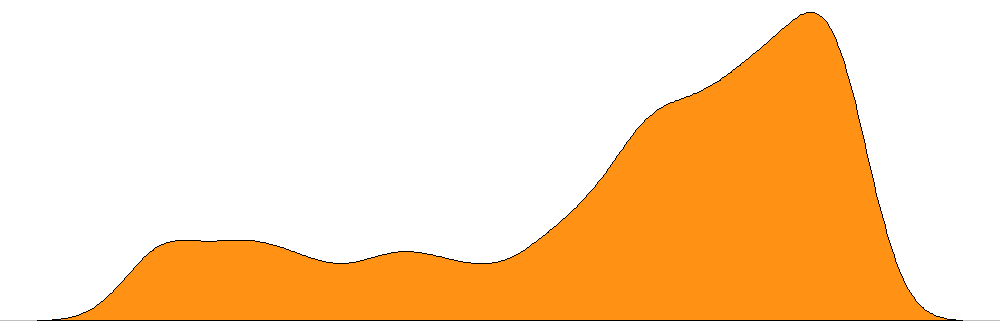
\includegraphics[height=1em]{tinytable_assets/idkw3ss7dtaehv6mshzwwl.png} \\
Linkages to China & 5154 & 0.08 & 0.05 & 0.08 & 0.00 & 0.48 & 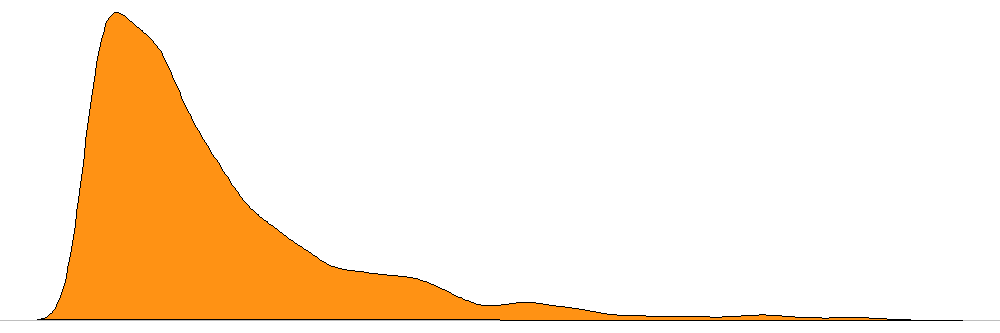
\includegraphics[height=1em]{tinytable_assets/idgbl0sn5x5im94irfzhyq.png} \\
GDP per capita & 5190 & 8.20 & 8.16 & 1.58 & 4.37 & 11.81 & 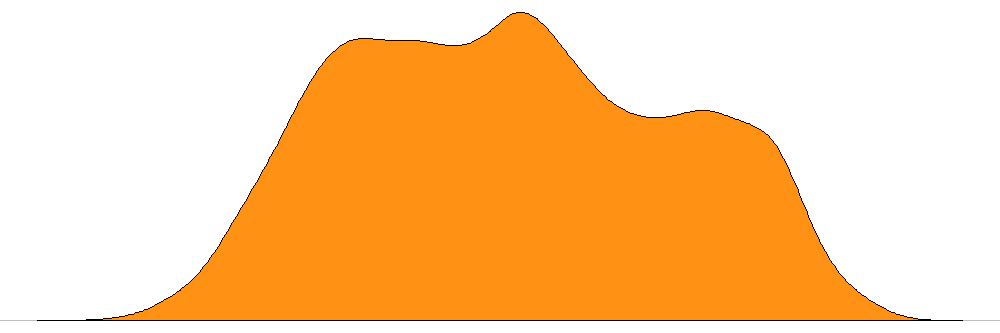
\includegraphics[height=1em]{tinytable_assets/iduvca3az1vb55iagqjao4.png} \\
Natural resources & 4679 & 7.74 & 2.68 & 11.35 & 0.00 & 88.59 & 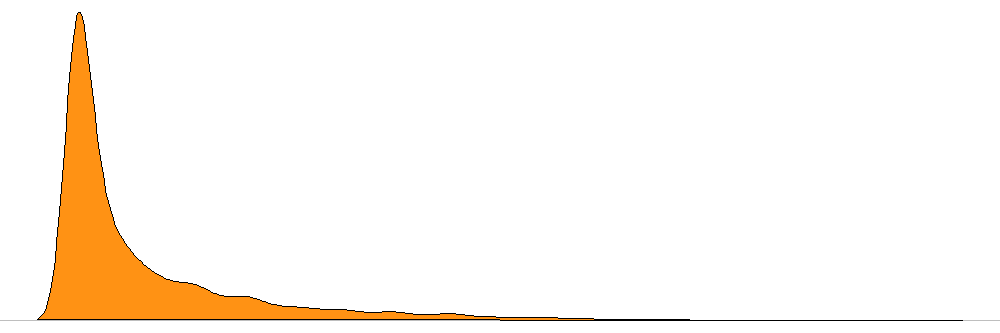
\includegraphics[height=1em]{tinytable_assets/id2fj7dkybom42ciuf8nxw.png} \\
Aid & 5213 & 4.25 & 0.78 & 8.01 & 0.00 & 113.13 & 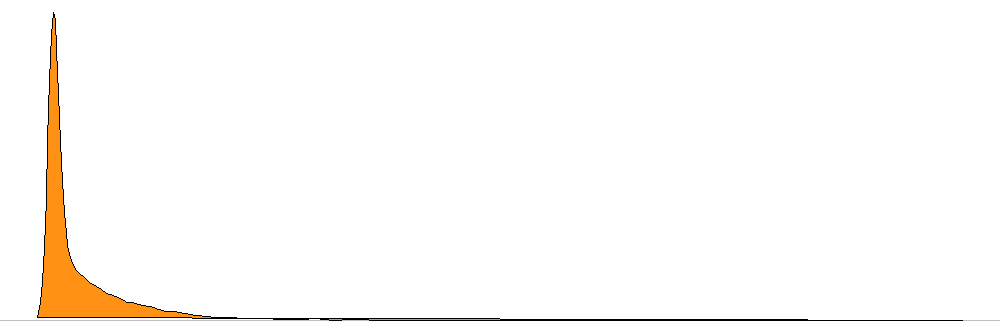
\includegraphics[height=1em]{tinytable_assets/idsk9x35wnd8lbeg36z6ir.png} \\
Linkages to the West & 5154 & 1.08 & 0.68 & 1.08 & 0.03 & 5.32 & 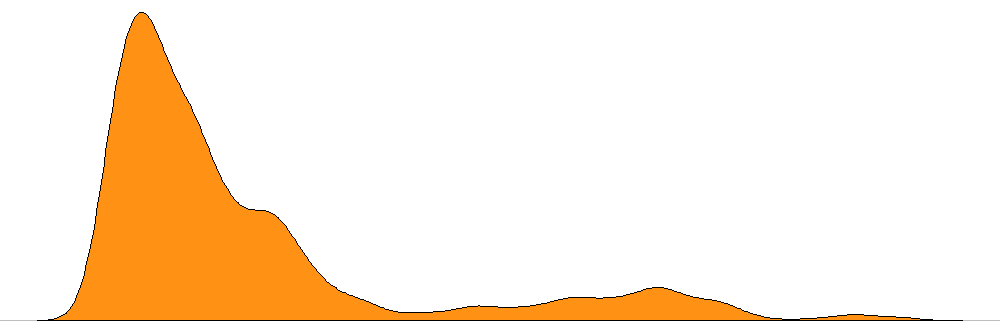
\includegraphics[height=1em]{tinytable_assets/id0blqnye1aky5vllx8gn6.png} \\
Regime & 5368 & 1.59 & 2.00 & 1.00 & 0.00 & 3.00 & 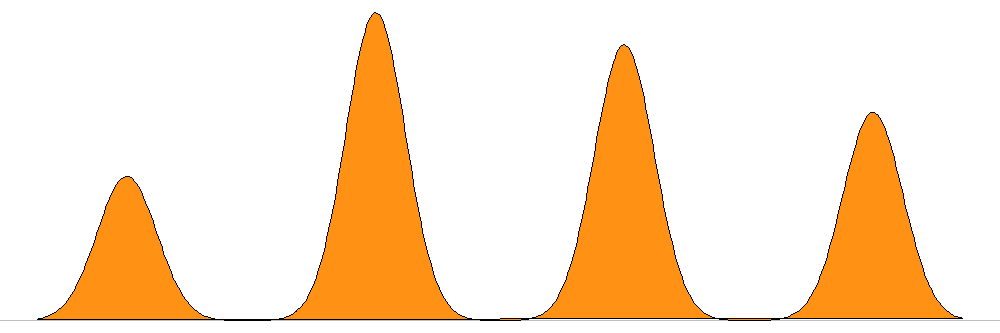
\includegraphics[height=1em]{tinytable_assets/idtplecxtx0acvwxi990hv.png} \\
\bottomrule
\end{tblr}
\end{table} 

\subsection{Challenges to inference}
While fixed effects solves many inference problems by removing time and unit constants, reducing unobserved variable bias. However, it is far from a panacea, and we need to be conscious of this fact. The first problem with using fixed effects is that there can still be \textit{unobserved heterogeneity} (\citeauthor{cunningham_causal_2021} \citeyear{cunningham_causal_2021}, Chapter 8, \citeauthor{hill_limitations_2020} \citeyear{hill_limitations_2020}, pp. 363-364). These are variable that vary across both unit and time. I try to account for this heterogeneity by including control variables, but there will always be a possibility that there is some unobserved heterogeneity; a risk that can only be mitigated to the best of one's ability.

A second challenge is that fixed-effects modelling can have \textit{low statistical power} \citep[pp. 361-362]{hill_limitations_2020}. Taking the within variation might limit information and this makes estimation harder. My linkage variable has a mean of 0.08, which is quite small. So, this could be a challenge. I still consider there to be enough variation to be useful, but this is something to keep in mind.

The last major concern of fixed-effects is that \textit{coefficients are harder to interpret} \citep[pp. 364-365]{hill_limitations_2020}. This is especially so for the two-way fixed effect model I use here. To try to make it easier for the reader I will use examples, to show how the coefficients might be interpreted.

\subsection{The models}
Fixed effects solve the problem where variables that are fixed over time and country influences the results. The last hurdle is to remove effects caused by variables that varies over both time and units. To do this I include the controls for GDP per capita, natural resources rents, aid, and linkages to the West. Including these should remove any spurious effects that might cause bias when estimating the relationship between linkages to China and freedom of expression. The final models are represented in the two equations below.
\begin{align} \label{equ:h1}
    freedom_{it+1} =\, & \beta_1  linkages_{it} + \beta_2 log(gdppc)_{it} + \beta_3 rents_{it} + \beta_4aid_{it} + \nonumber\\
    & \beta_5 west_{it} + \beta_6  factor(regime)_{it} + \chi_1 country_t + \chi_2 time_i + \epsilon_{it}
\end{align}
In Equation \ref{equ:h1} the freedom of expression variable with a one-year lead is a function of  linkages to China, the log-transformed GDP per capita, rents, aid, linkages to the west, regime type, and an error term.

When working with hypotheses two, we need a slightly different model from the one above. Instead of including the regime variable as an independent term, we furnish the models with an interaction term between the linkage variable and the factorised regime variable. This makes it possible to see the effect of linkages on different regime types. The interaction model is shown in Equation \ref{equ:h2}:
\begin{align} \label{equ:h2}
    freedom_{it+1} =\, & \beta_1 linkages_{it} + \beta_2 factor(regime)_{it} + \beta_2 log(gdppc)_{it} + \beta_3 rents_{it} + \nonumber\\
    & \beta_4 aid_{it} + \beta_5 west_{it} + \beta_6 (linkages * factor(regime)) + \nonumber\\
    & \chi_1 country_t +\chi_2 time_i + \epsilon_{it}
\end{align}